\documentclass{article} 
\usepackage{graphicx}
\usepackage{moreverb}
\usepackage{natbib}
\usepackage{url}

\linespread{1.5}
\begin{document} 
\nocite{*}
\begin{titlepage}
\title{Resource Allocation In Cloud Computing}
\author{ Hossam Saraya}
\maketitle

\vspace{100 pt}
\begin{abstract}
 Cloud computing is becoming one of the major concerns in the IT field. Cloud computing provides an on-demand network access to configurable computing resources and allows consumers and businesses to use applications without installation and access their personal files at any computer with internet access. This technology allows for much more efficient computing by centralizing resources such as storage, memory, processing and bandwidth. In order for a cloud based environment to be efficient, it has to manage the resources efficiently among nodes in the cloud. This paper proposes an algorithm for an optimal resource allocation in cloud computing environments to ensure an efficient resource management.
\end{abstract}
\end{titlepage}

\tableofcontents 
\newpage


\section{Introduction}
\subsection{Why Cloud Computing?}
People and enterprises started migrating to cloud computing for many reasons. First of all, cloud computing/hosting is cheaper than the classic hosting we used to see in the past because when in a cloud, a client is rented the needed resources in pay-as-you-go fashion. That means, the client will never have to pay for a 100GB server if he is not sure of how much of space he needs as the disk space is allocated dynamically on demand. Moreover, in cloud hosting, the client does not have to maintain the machine because simply this machine is virtual. The real maintenance, patching, administration is done automatically by the cloud provider. 

Cloud computing services are rapidly gaining in popularity. They allow the user to rent, only at the time when needed, only a desired amount of computing resources (processing ability and storage capacity) out of a huge mass of distributed computing resources without worrying about the locations or internal structures of these resources. The popularity of cloud computing owes to the increase in the network speed, and to the fact that virtualization and grid computing technologies have become commercially available. It is anticipated that enterprises will accelerate their migration from building and owning their own systems to renting cloud computing services because cloud computing services are easy to use, and can reduce both business costs and environmental loads [1]. Cloud computing can be categorized into three models: IaaS (Infrastructure as a service), PaaS (Platform as a service), SaaS (Software as a service). In this paper, we will be talking about IaaS and how to manage the available resources efficiently from the cloud provider perspective.

In IaaS, cloud providers offer consumers Internet access to virtual machines that are in fact a collection of real computers acting together behind the curtains in a data center. For the consumers to deploy applications, they have to connect to the cloud, install an operating system on their virtual machine, and behave normally like they would do in the case of a personal computer. In IaaS model, the consumer is responsible for maintaining, managing their virtual machine. The virtual machine resources like CPU power, Storage, RAM are provided on-demand to the consumer. From the cloud provider point of view, many consumers submit requests to allocate resources like CPU Power, RAM, Storage for use in their virtual machines. Therefore, the cloud provider must have an efficient way to allocate resources to many clients by filling their requests without losing money (economic allocation). In this paper, we will be only concerned with disk space (Storage) allocation. We will suggest a suitable algorithm and then simulate it on CloudSim which is an architecture for cloud simulation. We will consider factors like time, distance, available resources while allocating resources to the consumers. 


\subsection{Tools we will be using}
\subsubsection{Python}
Python is a general-purpose, high-level programming language whose design philosophy emphasizes code readability, remarkable power and its standard library is large and comprehensive.
Python supports multiple programming paradigms, primarily but not limited to object-oriented, imperative and, to a lesser extent, functional programming styles. It features a fully dynamic type system and automatic memory management, similar to that of Scheme, Ruby, Perl, and Tcl. Like other dynamic languages, Python is often used as a scripting language, but is also used in a wide range of non-scripting contexts. Using third-party tools, Python code can be packaged into standalone executable programs. Python interpreters are available for many operating systems.
The reference implementation of Python (CPython) is free and open source software and has a community-based development model, as do nearly all of its alternative implementations. CPython is managed by the non-profit Python Software Foundation \cite{python}.

\subsubsection{Java}
Java is a programming language originally developed by James Gosling at Sun Microsystems (which has since merged into Oracle Corporation) and released in 1995 as a core component of Sun Microsystems' Java platform. The language derives much of its syntax from C and C++ but has a simpler object model and fewer low-level facilities. Java applications are typically compiled to bytecode (class file) that can run on any Java Virtual Machine (JVM) regardless of computer architecture. Java is a general-purpose, concurrent, class-based, object-oriented language that is specifically designed to have as few implementation dependencies as possible. It is intended to let application developers "write once, run anywhere" (WORA), meaning that code that runs on one platform does not need to be recompiled to run on another. Java is currently one of the most popular programming languages in use, particularly for client-server web applications, with a reported 10 million users \cite{java}.

\subsubsection{Eclipse}
Eclipse is a multi-language software development environment comprising an integrated development environment (IDE) and an extensible plug-in system. It is written mostly in Java. It can be used to develop applications in Java and, by means of various plug-ins, other programming languages including Ada, C, C++, COBOL, Perl, PHP, Python, R, Ruby (including Ruby on Rails framework), Scala, Clojure, Groovy and Scheme. It can also be used to develop packages for the software Mathematica. Development environments include the Eclipse Java development tools (JDT) for Java, Eclipse CDT for C/C++, and Eclipse PDT for PHP, among others \cite{eclipse}.

\newpage
\section{Related Work}
We are not the first to propose an algorithm for resource allocation in cloud computing, there are already many approaches being used by cloud providers like Amazon EC2, Google App Engine and GoGrid. There are numerous research papers regarding the problem of resource allocation that have been studied. In this section, we analyze the great work of other authors who contributed to the field of cloud computing.

\subsection{Optimal Joint Multiple Resource Allocation Method for Cloud Computing Environments}
This paper shows in details the evolution of cloud computing possibilites due to the increase of the available network bandwidth. This paper suggests an algorithm to allocate multiple resource types simultaneously, later on in the same paper, a fair-allocation algorithm is suggested by the author. The authors assumed non-delay system with static resources in their research. Their objective is to maximize the resource utilization while allocating resources (minimize the wasted resrouces). In their paper, they are only considering two types of resources: Bandwidth and processing power. As the size of the required resources can't be generalized and it's always different, optimilaity in resource allocation is very hard be achieved if we consider only one random type of resources while allocation. The figure below illustrates two cases, in the case 1, only processing ability is considered in the selection of the data center. Unlike case 1, case 2 considers both processing ability and bandwidth in the data center selection. In the first case, a resource request requires a certain amount of bandwidth and processing power, but the request will be rejected because our cluster is in a deadlock state, center 1 has enough bandwidth for the request, but it doesn't have the required processing ability. Center 2 has enough processing power but not enough bandwidth. In the previous case, we saw how we can reach a deadlock state if we only consider one type of resources. To overcome the deadlock problem, multiple resource types should be considered when allocating resources to customers, this is demonstrated in case 2 in the figure below. 

\begin{figure}[htb]
\centering
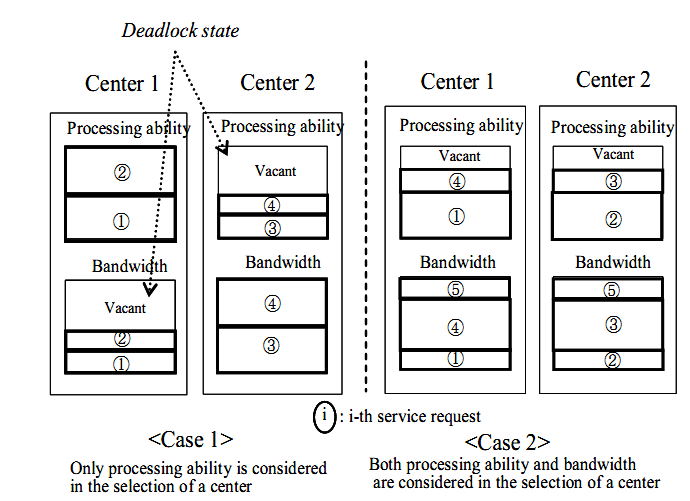
\includegraphics[width=0.8\textwidth]{pasted1}
\end{figure}

The authors then shows that it's difficult to follow the method suggested above which considers many types of resources while allocating. They then suggest select the resource type which has the biggest impact on resource allocation and they called it “Identified resource”. Identified resource will be the only resource type that will contribute in the data-center selection process. This method adopts Best-Fit approach and aims to reserve as much as possible for future requests that may acquire larger size of processing power or bandwidth. To overcome the possibility of deadlocks like discuessed above in case 1, they proposed using round-robin method in which the centers are selected in turn in a predefined order.

The resource type that has the bigger impact on our resource pool will be selected as the identified resource. In other words, the resource type that requires the largest proportionate size of resource, comparing the required resource size with the maximum size for each resource type is selected as the identified resource. Then the center with the least available amount of the required size is selected from among k centers. (Best-Fit)\cite{optimaljoint}

\section{Resource Allocation}
A typical cloud provider has one or many data centers, in these data center there are physical servers which acts as the cloud's physical layer. On top of the physical layer, there are virtual machines that act as the cloud virtualization layer. The user usually is provided a web interface to request virtual machines with the needed specifications (RAM,CPU,Storage). Resource allocation in cloud computing happens when a new user requests a virtual machine with a set of specifications (RAM,CPU,Storage), the user usually does that through the web interface of the cloud provider. Another scenario is when the user already has a hosted virtual machine in one of the cloud provider's data centers, and he requests to customize it. eg: (get more Storage or RAM). In this chapter, different approaches for resource allocation will be covered along with a comparison between them in different scenarios.

The cloud provider may follow one of the following paradigms for resource allocation. 


\begin{itemize}
\item Immediate Allocation
\item Immediate Allocation with Placement Policies
\item BE (Best Effort Allocation)
\item AR (Advanced Reservation Allocation)
\item DLS (DeadLine Senstive Allocation)
\end{itemize}
\newpage

\subsection{Immediate Allocation}
Immediate allocation is useful when the allocation request arises for resources and it needs immediate attention. If the physical layer doesn't have the requested resources, the request is cancelled by the resource scheduler. Immediate allocation is used in OpenNebula an open source tool that supports IaaS model by managing virtual machines (VMs), as an abstraction of infrastructure, for private, public and hybrid clouds.
\begin{center}
\begin{verbatimtab}
if requested resource are available then: 
	allocate resources for the client 
else: 	
	reject request
\end{verbatimtab}
\end{center}

\subsection{Best Effort Allocation}
In Best Effort allocation, requests are inserted into a queue and treated by the resource scheduler in FIFO manner on the availability of resources.

\begin{verbatimtab}
function HandleRequest(Request):
	requestQueue.queue(Request)

function ScheduleResources: 
	req = requestQueue.dequeue()
	while( req != null) 	
		if (req.resources is available): 	
			allocate resources to the client 
			req = resourceQueue.dequeue()
\end{verbatimtab}
\newpage

\subsection{Immediate Allocation with placement policies }
This approach of allocation is similar to this discussed in 3.1. The only difference here that in allocation we follow one of the following policies while allocating:

\subsubsection{Packing}
Packing policy minimizes the number of cluster nodes in use by using those nodes with more VMs running first \cite{optimaljoint}.

\subsubsection{Striping}
Striping policy maximizes the resources available to VMs in a node by using those nodes with less VMs running first \cite{optimaljoint}.

\subsubsection{Load-aware Policy}
Striping policy minimizes the CPU power available to VMs in a node by using those nodes with more free CPU first \cite{optimaljoint}.

\subsection{Advanced Reservation Allocation}
In this approach of allocation. Each request must have a start time, end time for the required resources. The scheduler then allocates the resources -if avalailable- in the requested time slot \cite{optimaljoint}.

\subsection{Deadline Senstive Allocation}
In Deadline Sensitive Allocation, Each request has a deadline, if the request can not be fulfilled before it's deadline, then it's rejected by the resource scheduler \cite{optimaljoint}.
\newpage


\section{Implementation}

\section{Conclusion}

\newpage
\bibliographystyle{plain}
\bibliography{references}

\end{document}

 
